\documentclass{beamer}
\usepackage{pdfpages}
%Imports and customization
\usepackage{tikz}
\usepackage{graphicx}
\usepackage{tikz-feynman}
\usepackage{ulem}
\usepackage{colortbl}
\graphicspath{ 
    {./images/}
}

\beamertemplatenavigationsymbolsempty
\setbeamertemplate{sidebar right}{}
\setbeamertemplate{footline}{
    \hfill\usebeamertemplate***{navigation symbols}
    \hspace{1cm}\insertframenumber{}/\inserttotalframenumber
}
\setbeamertemplate{caption}{\raggedright\insertcaption\par}
\setbeamersize{text margin left=4mm,text margin right=4mm} 

\setbeamerfont{itemize/enumerate body}{size=\scriptsize}
\setbeamerfont{itemize/enumerate subbody}{size=\scriptsize}
\setbeamerfont{itemize/enumerate subsubbody}{size=\scriptsize}


%Custom Macros
\newcommand{\statwarn}{
    \tiny \color{red} Absolute numbers here mean NOTHING. Plots are based on small (100k events) samples, and are highly biased. All that matters is relative position!
}


% WARNING: When using these commands, the image argument must
% NOT have spaces between itself and the braces
\newcommand{\fullscreenimage}[2]{
    \frame{
        \frametitle{#1} 
        \begin{figure}
        \includegraphics[height=0.9\textheight,width=\textwidth,keepaspectratio]{#2}
        \end{figure}
    }
}


\newcommand{\importpdf}[3]{
    \frame{
        \begin{columns}\column{\dimexpr\paperwidth-10pt}
        \begin{figure}
        \includegraphics[page=#2,height=0.8\textheight,width=\textwidth,keepaspectratio]{#1}
        \end{figure}

        {\tiny #3}
        \end{columns}
    }
}


\newcommand{\displayone}[3]{
    \frame{
        \frametitle{#1} 
        \begin{columns}
            \begin{column}{0.5\textwidth}
                #2
            \end{column}
            \begin{column}{0.5\textwidth}
                \begin{figure}
                    \includegraphics[width=\linewidth,height=\textheight,keepaspectratio]{#3}
                \end{figure}
            \end{column}
        \end{columns}
    }
}

\newcommand{\displayonelarge}[3]{
    \frame{
        \frametitle{#1} 
        \begin{columns}
            \begin{column}{0.3\textwidth}
                #2
            \end{column}
            \begin{column}{0.7\textwidth}
                \begin{figure}
                    \includegraphics[width=\linewidth,height=0.8\textheight,keepaspectratio]{#3}
                \end{figure}
            \end{column}
        \end{columns}
    }
}


\newcommand{\displaytwo}[4]{
    \frame{
        \frametitle{#1} 
        #2
        \begin{columns}
            \begin{column}{0.5\textwidth}
                \begin{figure}
                    \includegraphics[width=\linewidth,height=\textheight,keepaspectratio]{#3}
                \end{figure}
            \end{column}
            \begin{column}{0.5\textwidth}
                \begin{figure}
                    \includegraphics[width=\linewidth,height=\textheight,keepaspectratio]{#4}
                \end{figure}
            \end{column}
        \end{columns}
    }
}

\newcommand{\displaytwocaption}[6]{
    \frame{
        \frametitle{#1} 
        #2
        \begin{columns}
            \begin{column}{0.5\textwidth}
                \begin{figure}
                    \includegraphics[width=\linewidth,height=\textheight,keepaspectratio]{#3}
                    \caption{#4}
                \end{figure}
            \end{column}
            \begin{column}{0.5\textwidth}
                \begin{figure}
                    \includegraphics[width=\linewidth,height=\textheight,keepaspectratio]{#5}
                    \caption{#6}
                \end{figure}
            \end{column}
        \end{columns}
    }
}

\newcommand{\displaytwoVcaption}[6]{
    \frame{
        \begin{columns}
            \begin{column}{0.5\textwidth}
                \frametitle{#1} 
                #2
            \end{column}
            \begin{column}{0.5\textwidth}
                \begin{figure}
                    \includegraphics[width=\linewidth,height=0.3\textheight,keepaspectratio]{#3}
                    \caption{#4}
                \end{figure}

                \begin{figure}
                    \includegraphics[width=\linewidth,height=0.3\textheight,keepaspectratio]{#5}
                    \caption{#6}
                \end{figure}
            \end{column}
        \end{columns}
    }
}


\newcommand{\displaythree}[5]{
    \frame{
        \begin{columns}[T]
            \begin{column}{0.4\textwidth}
                {\usebeamercolor[fg]{title} \insertframetitle{#1} }\\
                \vspace{5mm}
                #2
            \end{column}
            \begin{column}{0.4\textwidth}
                \begin{figure}
                    \includegraphics[width=\linewidth,height=\textheight,keepaspectratio]{#3}
                \end{figure}
            \end{column}
        \end{columns}
        \begin{columns}[T]
            \begin{column}{0.4\textwidth}
                \begin{figure}
                    \includegraphics[width=\linewidth,height=\textheight,keepaspectratio]{#4}
                \end{figure}
            \end{column}
            \begin{column}{0.4\textwidth}
                \begin{figure}
                    \includegraphics[width=\linewidth,height=\textheight,keepaspectratio]{#5}
                \end{figure}
            \end{column}
        \end{columns}
    }
}


\newcommand{\displayfour}[5]{
    \frame{
        \frametitle{#1} 
        \begin{columns}[T]
            \begin{column}{0.4\textwidth}
                \begin{figure}
                    \includegraphics[width=\linewidth,height=\textheight,keepaspectratio]{#2}
                \end{figure}
            \end{column}
            \begin{column}{0.4\textwidth}
                \begin{figure}
                    \includegraphics[width=\linewidth,height=\textheight,keepaspectratio]{#3}
                \end{figure}
            \end{column}
        \end{columns}
        \begin{columns}[T]
            \begin{column}{0.4\textwidth}
                \begin{figure}
                    \includegraphics[width=\linewidth,height=\textheight,keepaspectratio]{#4}
                \end{figure}
            \end{column}
            \begin{column}{0.4\textwidth}
                \begin{figure}
                    \includegraphics[width=\linewidth,height=\textheight,keepaspectratio]{#5}
                \end{figure}
            \end{column}
        \end{columns}
    }
}


\newcommand{\pstrike}[2]{
    \only<-\the\numexpr#1-1>{#2}
    \only<#1->{\sout{#2}}
}


\newcommand{\announcesection}[1]{
    \section{#1}
    \frame{
        \begin{center}
            {\huge #1} 
        \end{center}
    }
}

\newcommand{\kvv}{\kappa_{2V}}
\newcommand{\kl}{\kappa_{\lambda}}
\newcommand{\kv}{\kappa_{V}}

\newcommand{\fkvv}[1]{\kappa_{2V,#1}}
\newcommand{\fkl} [1]{\kappa_{\lambda,#1}}
\newcommand{\fkv} [1]{\kappa_{V,#1}}

\newcommand{\importpdfwpages}[3]{
    \foreach \pageN in {#2,...,#3}{
        \importpdf{#1}{\pageN}{}
    }
}

\newcommand{\hyper}[2]{{\color{blue}\href{#1}{#2}}}



%Begin Presentation
\begin{document}
    \setbeamercolor{background canvas}{bg=}
    \title{SMU ATLAS Status Update\\VBF HH MC Combination Studies}
    \author{Chris Milke}
    \date{17 June, 2021}

    \frame{\titlepage}
    \frame{\frametitle{Overview} \tableofcontents}

    % Intro
    \section{ATLAS Di-Higgs Analysis and MC Sample Combinations}

\displaytwocaption{ATLAS Di-Higgs Analysis}{
    Working with Di-Higgs analysis to discover HH process.
}
{ggF_diagrams}
{$\sigma_{ggF \rightarrow HH}=33.5^{+2.4}_{-2.8}$fb at NNLO}
{vbf-hh_diagrams}
{$\sigma_{VBF \rightarrow HH}=1.73\pm0.04$fb at N\textsuperscript{3}LO}


    % show diagrams with terms, then show squaring
\frame{
    \frametitle{3D Coupling Dependence}

    {\small
        We need large coverage of the 3-coupling parameter space, but signal samples are computationally expensive to produce.
        We can use the underlying math of field theory to create a shortcut:
    }

    \begin{figure}
    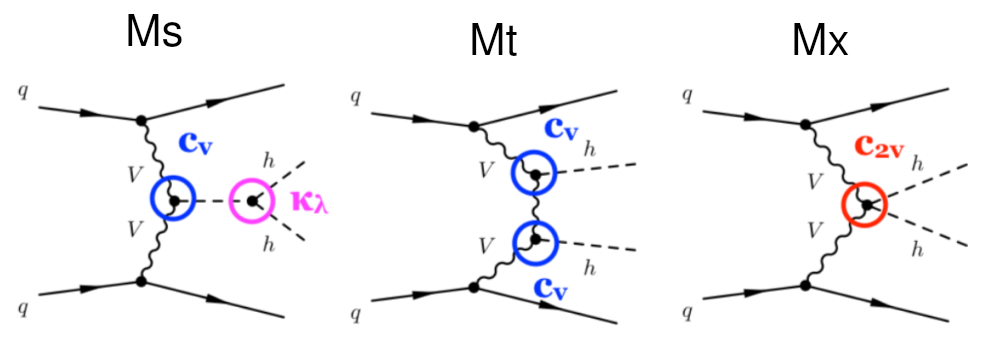
\includegraphics[width=0.5\linewidth,height=0.6\textheight,keepaspectratio]{vbf-hh_diagrams2b}
    \end{figure}
    $ \sigma = |A|^2 = | \kv \kl M_s + \kv^2 M_t + \kvv M_x |^2 = $

    \vspace{5mm}

    $ \kv^2 \kl^2 M_s^2 + \kv^4 M_t^2 + \kvv^2 M_x^2 
    + \kv^3 \kl (M_s^* M_t + M_t^* M_s) 
    + \kv \kl \kvv (M_s^* M_x + M_x^* M_s ) 
    + \kv^2 \kvv (M_t^* M_x + M_x^* M_t )$

    \vspace{5mm}

    $ \sigma = \kv^2 \kl^2 a_1 + \kv^4 a_2 + \kvv^2 a_3 + \kv^3 \kl a_4 + \kv \kl \kvv a_5 + \kv^2 \kvv a_6 $
}

% 6 variables, six equations, make a mess
\frame{
    \frametitle{6 Unknowns: Solve With 6 Equations}

    \vspace{5mm}

    \foreach \index in {1,2,3,4,5,6}{
        { \small $ \sigma_\index = \fkv{\index}^2 \fkl{\index}^2 a_1 + \fkv{\index}^4 a_2 + \fkvv{\index}^2 a_3 + \fkv{\index}^3 \fkl{\index} a_4 + \fkv{\index} \fkl{\index} \fkvv{\index} a_5 + \fkv{\index}^2 \fkvv{\index} a_6 $ }

        \vspace{5mm}
    }
}

% convert to matrix, show nice matrix solution
\frame{
    \frametitle{Linear Algebra Makes this Simple}

    \begin{columns}[T]
        \begin{column}{0.18\textwidth}
            $ \vec{\sigma} = \begin{pmatrix} \sigma_1 \\ \sigma_2 \\ \sigma_3 \\ \sigma_4 \\ \sigma_5 \\ \sigma_6 \end{pmatrix} $
        \end{column}
        \begin{column}{0.15\textwidth}
            $ \vec{a} = \begin{pmatrix} a_1 \\ a_2 \\ a_3 \\ a_4 \\ a_5 \\ a_6 \end{pmatrix} $
        \end{column}
        \begin{column}{0.25\textwidth}
            $ \vec{f} = \begin{pmatrix} \kv^2 \kl^2 \\ \kv^4 \\ \kvv^2 \\ \kv^3 \kl \\ \kv \kl \kvv \\ \kv^2 \kvv \end{pmatrix} $
        \end{column}
        \begin{column}{0.4\textwidth}
            $ F = \begin{pmatrix}
                \vec{f}(\fkvv{1}, \fkl{1}, \fkv{1}) \\
                \vec{f}(\fkvv{2}, \fkl{2}, \fkv{2}) \\
                \vec{f}(\fkvv{3}, \fkl{3}, \fkv{3}) \\
                \vec{f}(\fkvv{4}, \fkl{4}, \fkv{4}) \\
                \vec{f}(\fkvv{5}, \fkl{5}, \fkv{5}) \\
                \vec{f}(\fkvv{6}, \fkl{6}, \fkv{6}) \\
            \end{pmatrix} $
        \end{column}
    \end{columns}

    \vspace{10mm}

    $ \vec{\sigma} = F \bullet \vec{a} \; \Longrightarrow \; \vec{a} = F^{-1} \bullet \vec{\sigma} $

    \vspace{10mm}

    $ \boxed{ \sigma(\kvv,\kl,\kv) = \vec{f}(\kvv,\kl,\kv) \bullet F^{-1} \bullet \vec{\sigma} } $
}

    \section{Applying Linear Combination}

\frame{
    \frametitle{Linear Combination Using Post Reconstruction/Selection Samples}
    \begin{columns}
        \begin{column}{0.4\textwidth}
            \begin{center} 
            {\tiny Signal Sample Basis Set}

            \resizebox{0.2\textheight}{!}{ \begin{tabular}{ |l|l|l| }
                \hline
                \textbf {$\kappa_{2V}$} & \textbf {$\kappa_\lambda$} & \textbf {$\kappa_V$} \\
                \hline
                    1.  &   1. & 1.  \\
                    2.  &   1. & 1.  \\
                    1.5 &   1. & 1.  \\
                    0.  &   1. & 0.5 \\
                    1.  &   0. & 1.  \\
                    1.  &  10. & 1.  \\
                \hline
            \end{tabular}}
            \end{center}

        \end{column}
        \begin{column}{0.6\textwidth}
            \resizebox{0.8\textwidth}{!}{ \begin{minipage}{1.0\textwidth}
            Linear Combination Equation

            \vspace{10mm}

            {\tiny $
    \left(2 \kappa_{2V}^{2} - \frac{124 \kappa_{2V} \kappa_{V}^{2}}{9} + \frac{61 \kappa_{2V} \kappa_{V} \kappa_{\lambda}}{9} + \frac{106 \kappa_{V}^{4}}{9} - \frac{17 \kappa_{V}^{3} \kappa_{\lambda}}{3} - \frac{\kappa_{V}^{2} \kappa_{\lambda}^{2}}{9}\right) \left|{A{\left(1,1,1 \right)}}\right|^{2} +
$

$
    \left(2 \kappa_{2V}^{2} - 8 \kappa_{2V} \kappa_{V}^{2} + 3 \kappa_{2V} \kappa_{V} \kappa_{\lambda} + 6 \kappa_{V}^{4} - 3 \kappa_{V}^{3} \kappa_{\lambda}\right) \left|{A{\left(2,1,1 \right)}}\right|^{2} +
$

$
    \left(- 4 \kappa_{2V}^{2} + 20 \kappa_{2V} \kappa_{V}^{2} - 8 \kappa_{2V} \kappa_{V} \kappa_{\lambda} - 16 \kappa_{V}^{4} + 8 \kappa_{V}^{3} \kappa_{\lambda}\right) \left|{A{\left(1.5,1,1 \right)}}\right|^{2} +
$

$
    \left(16 \kappa_{2V} \kappa_{V}^{2} - 16 \kappa_{2V} \kappa_{V} \kappa_{\lambda} - 16 \kappa_{V}^{4} + 16 \kappa_{V}^{3} \kappa_{\lambda}\right) \left|{A{\left(0,1,0.5 \right)}}\right|^{2} +
$

$
    \left(\frac{4 \kappa_{2V} \kappa_{V}^{2}}{5} - \frac{4 \kappa_{2V} \kappa_{V} \kappa_{\lambda}}{5} + \frac{\kappa_{V}^{4}}{5} - \frac{3 \kappa_{V}^{3} \kappa_{\lambda}}{10} + \frac{\kappa_{V}^{2} \kappa_{\lambda}^{2}}{10}\right) \left|{A{\left(1,0,1 \right)}}\right|^{2} +
$

$
    \left(- \frac{\kappa_{2V} \kappa_{V}^{2}}{45} + \frac{\kappa_{2V} \kappa_{V} \kappa_{\lambda}}{45} + \frac{\kappa_{V}^{4}}{45} - \frac{\kappa_{V}^{3} \kappa_{\lambda}}{30} + \frac{\kappa_{V}^{2} \kappa_{\lambda}^{2}}{90}\right) \left|{A{\left(1,10,1 \right)}}\right|^{2}
$
}
            \end{minipage}}
        \end{column}
    \end{columns}
}

\displaythree{Validity of Sample Combinations}
{ \small 
    Combining the six basis samples allows for modelling of distributions for any coupling values.
}
{reco_mHH_cvv1p0cl2p0cv1p0_ancient}
{reco_mHH_cvv0p0cl1p0cv1p0_ancient}
{reco_mHH_cvv4p0cl1p0cv1p0_ancient}

\displayonelarge{Full 2D Exclusion Plot ($\kv=1$)}{
    Using the distribution of the diHiggs invariant mass, $m_{HH}$,
    we can set expected limits on the HH cross-section as a function
    of the couplings $\kvv$ and $\kl$.
}{2D_scan_2D_scan_test01_noMC16e_samps_vbf_pd_1617_c1v1.0_exclusion}

    \section{Negative Weight Sledgehammer}
\frame{
    \frametitle{Finding a Basis with a Better Metric}
        \begin{columns} \begin{column}{0.5\textwidth}
    \begin{center} 
        (70 Possible Combinations of 6... 30 if requiring SM point)

        \resizebox{0.3\textheight}{!}{\begin{tabular}{ |l|l|l| }
            \hline
                \textbf {$\kappa_{2V}$} & \textbf {$\kappa_\lambda$} & \textbf {$\kappa_V$} \\
                \hline
                \rowcolor{red}   0   & 0   & 1   \\ % !!
                0   & 1   & 1   \\ 
                0.5 & 1   & 1   \\ 
                1   & 0   & 1   \\ 
                \rowcolor{red}   1   & 1   & 0.5 \\ % !!
                1   & 1   & 1   \\ 
                \rowcolor{red}   1   & 1   & 1.5 \\ % !!
                1   & 10  & 1   \\ 
                1   & 2   & 1   \\ 
                1.5 & 1   & 1   \\ 
                2   & 1   & 1   \\ 
                4   & 1   & 1   \\ 
                \rowcolor{green} 0   & 1   & 0.5 \\ % !!
                \hline
                \end{tabular}} \end{center}
    \end{column} \begin{column}{0.5\textwidth}
    \begin{center} 
    {\tiny Post-Reco Sample Basis Set}

    \resizebox{0.2\textheight}{!}{ \begin{tabular}{ |l|l|l| }
        \hline
            \textbf {$\kappa_{2V}$} & \textbf {$\kappa_\lambda$} & \textbf {$\kappa_V$} \\
            \hline
            1.  &   1. & 1.  \\
            2.  &   1. & 1.  \\
            1.5 &   1. & 1.  \\
            0.  &   1. & 0.5 \\
            1.  &   0. & 1.  \\
            1.  &  10. & 1.  \\
            \hline
            \end{tabular}}
    \end{center}

    \begin{figure}
    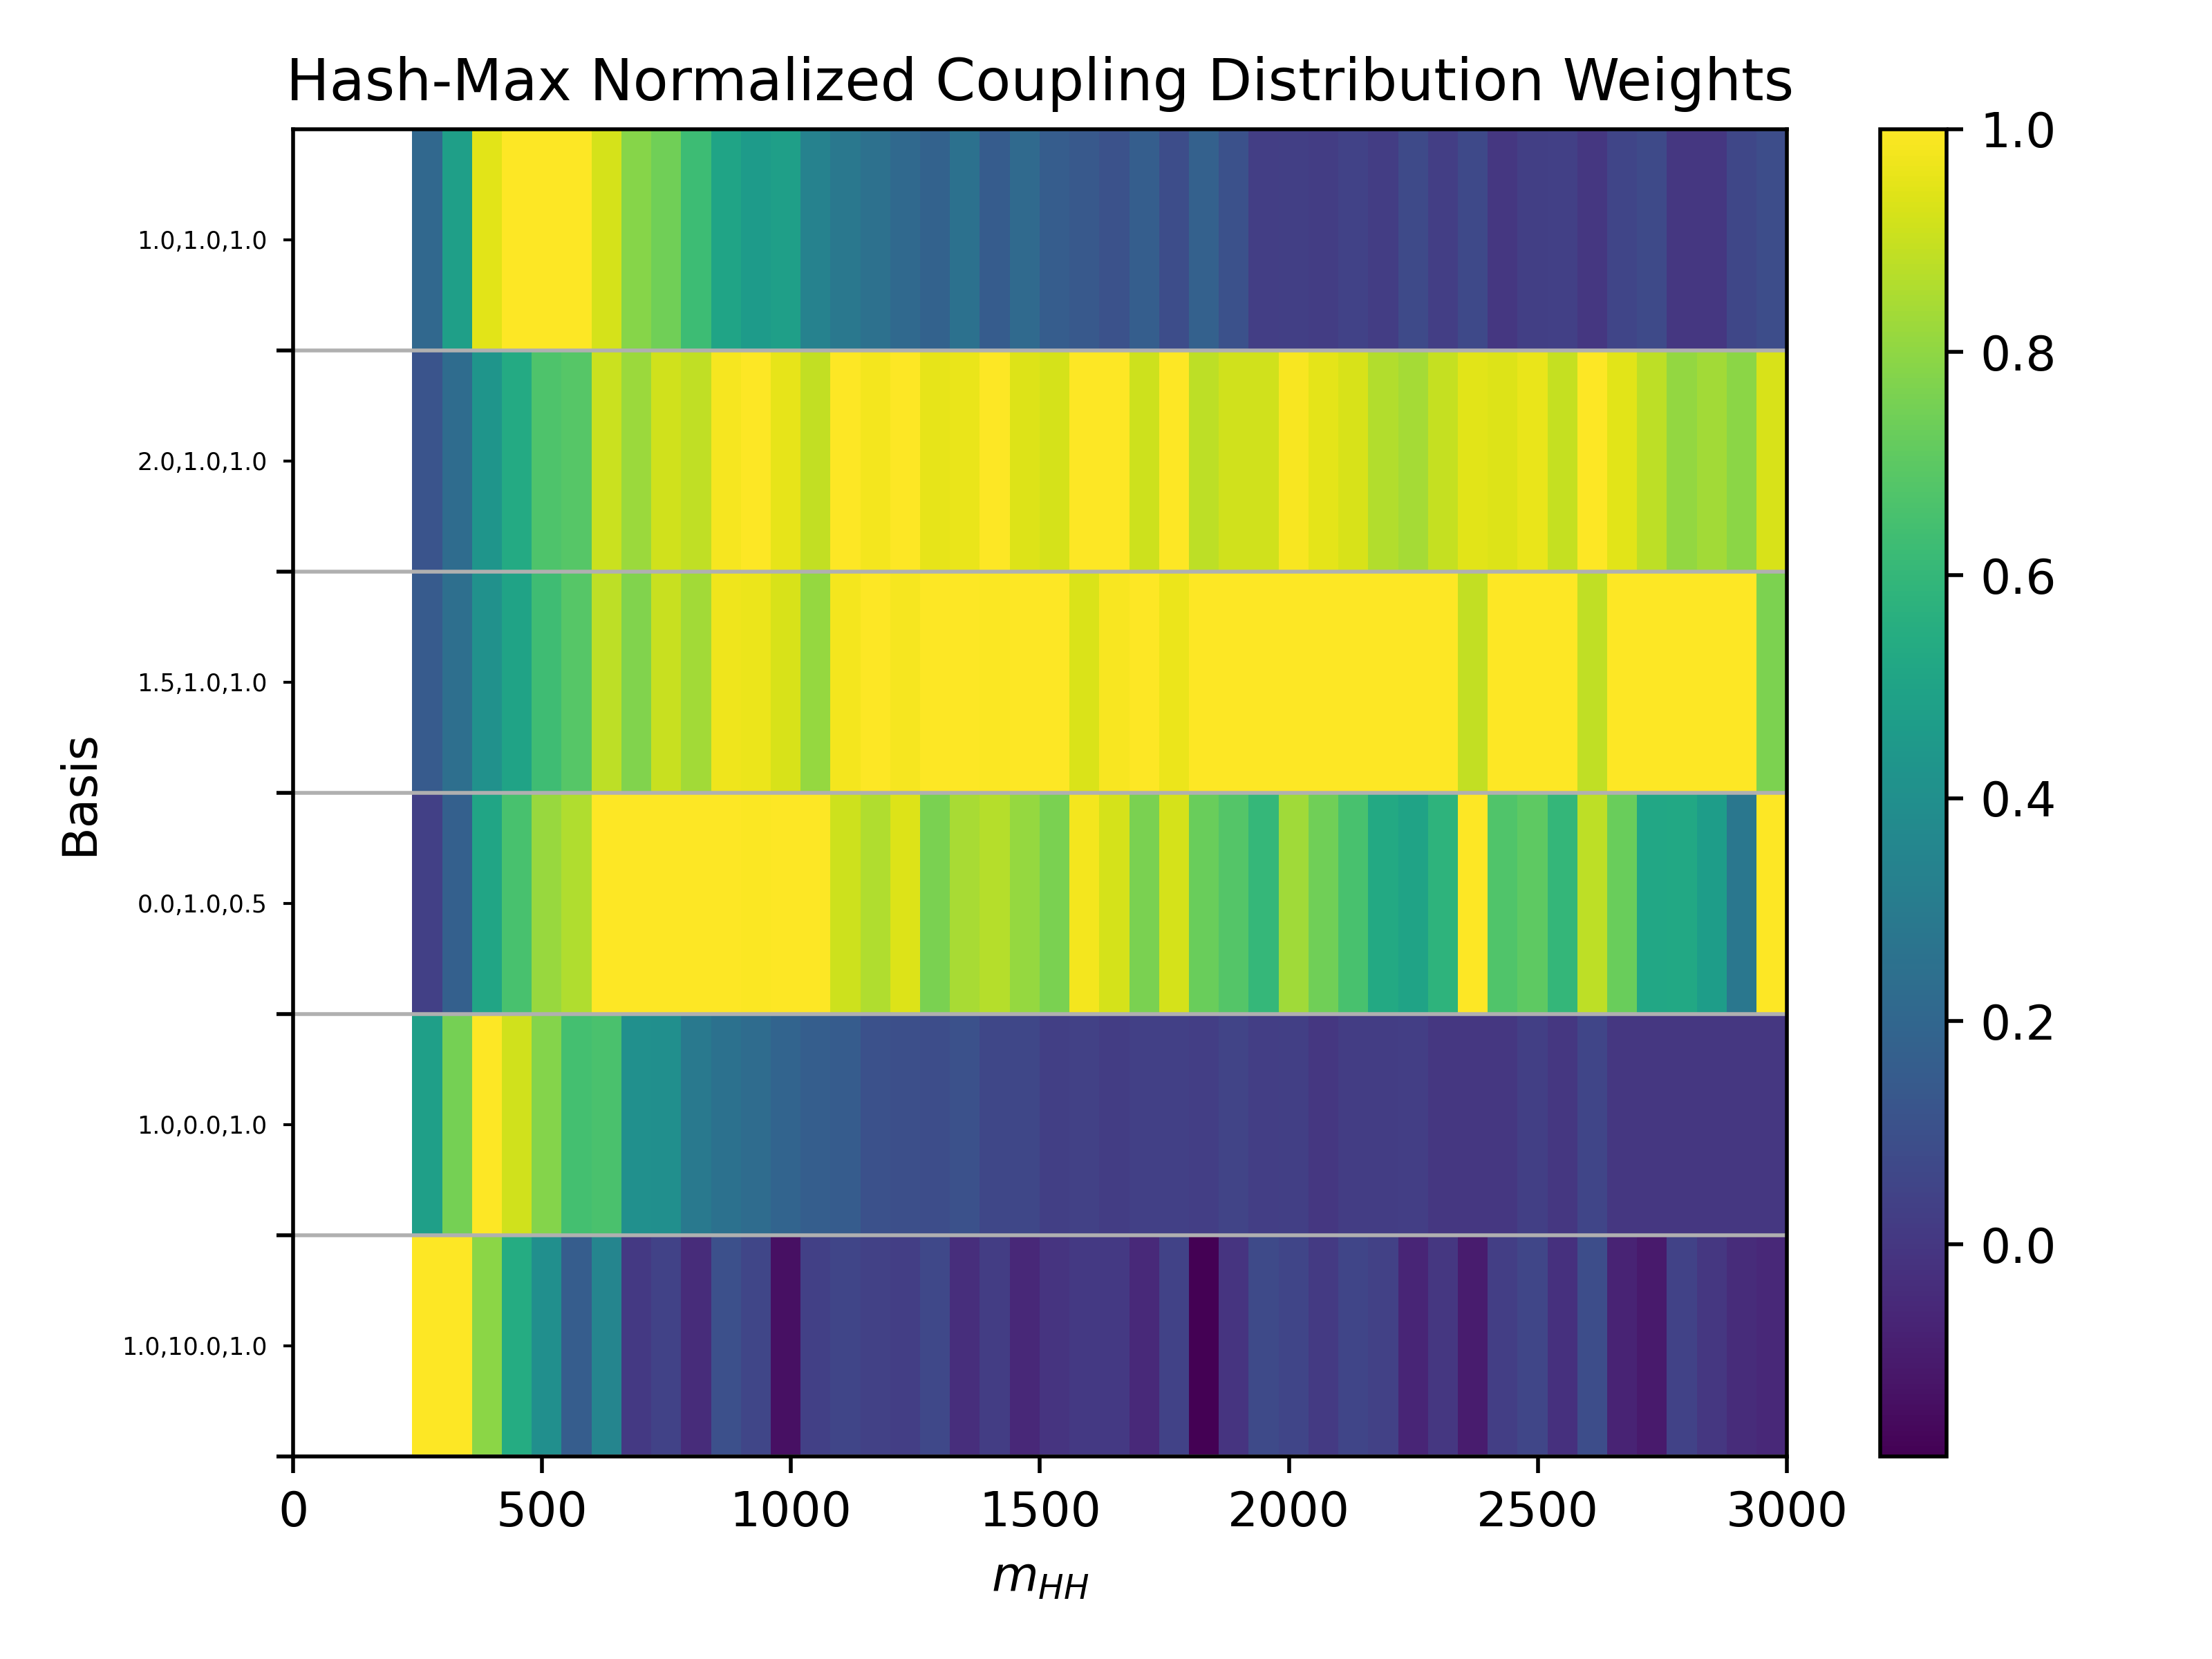
\includegraphics[width=\linewidth,height=\textheight,keepaspectratio]{coupling_scan_auto_chosen_reco_R0_hash_max}
    \end{figure}
    \end{column} \end{columns}
}

\displayonelarge{Negative Weights}{
    Negative weights can appear in the $m_{HH}$ combination. These are unphysical and should be avoided.
}{reco_mHH_cvv1p0cl2p0cv1p0_ancient}

\displayonelarge{Extreme Negative Weights}{
    In further regions of the $\kappa$ coupling space, these negative weights can be become dangerously common.
}{preview_reco_mHH_cvv0p0cl-9p0cv1p0_old}

\displayonelarge{Assessing Basis Performance via Negative Weight Integral}{
    Take the surface integral of the number of negative bins at each point at in the $\kappa$ parameter space (mutliplying by the $\kvv \times \kl$ ``area") as a general metric of performance.
}{negative_weights_rank027}

\displaythree{Negative-Weight Map of Different Bases}{
    Other bases show considerable improvement in the number of negative bins
}
{negative_weights_rank027}
{negative_weights_rank015}
{negative_weights_rank000}


\displaytwocaption{Limits with Negative-Weight Integral Rank-1 Basis}{
    Fewer negative weights results in a much more ``natural" limit boundary.

    Sharp edges and corners appear to have been a consequence of poor signal modelling.
}
{2D_scan_2D_scan_test01_noMC16e_samps_vbf_pd_1617_c1v1.0_exclusion}
{Using old basis}
{2D_scan_2D_scan_test02_newBasis_samps_vbf_pd_1617_c1v1.0_exclusion}
{Using new basis}

    \section{New MC Samples}

\frame{
    \frametitle{New MC Samples!}
    \begin{center} 
        {\small
            12 New MC Samples,\\
            619 Possible Combinations of 6,\\
            250 Include SM Sample
        }
        \vspace{5mm}

        \resizebox{0.8\textheight}{!}{
        \begin{columns} \begin{column}{0.3\textwidth}
            \begin{tabular}{ |l|l|l| }
                \hline
                \textbf {$\kappa_{2V}$} & \textbf {$\kappa_\lambda$} & \textbf {$\kappa_V$} \\
                \hline
                0    & 0   & 1   \\
                0    & 1   & 1   \\
                0.5  & 1   & 1   \\
                1    & 0   & 1   \\
                \hline
            \end{tabular}
        \end{column} \begin{column}{0.3\textwidth}
            \begin{tabular}{ |l|l|l| }
                \hline
                \textbf {$\kappa_{2V}$} & \textbf {$\kappa_\lambda$} & \textbf {$\kappa_V$} \\
                \hline
                1    & 1   & 0.5 \\
                1    & 1   & 1   \\
                1    & 1   & 1.5 \\
                1    & 10  & 1   \\
                \hline
            \end{tabular}
        \end{column} \begin{column}{0.3\textwidth}
            \begin{tabular}{ |l|l|l| }
                \hline
                \textbf {$\kappa_{2V}$} & \textbf {$\kappa_\lambda$} & \textbf {$\kappa_V$} \\
                \hline
                1    & 2   & 1   \\
                1.5  & 1   & 1   \\
                2    & 1   & 1   \\
                3    & 1   & 1   \\
                \hline
            \end{tabular}
        \end{column} \end{columns}
        }
    \end{center}
    \vspace{7mm}

    \begin{center} 
    Top 10 New Bases

    \resizebox{0.6\textwidth}{!}{
    \begin{tabular}{ |l|l|l|l|l|l|c| }
        \hline
            \textbf {Sample 1} & \textbf {Sample 2} & \textbf {Sample 3} &
            \textbf {Sample 4} & \textbf {Sample 5} & \textbf {Sample 6} &
            \textbf {Nweight Int}\\
            \hline
            (1, 1, 1) & (0.5, 1, 1) & (3, 1, 1) & (1, 2, 1 ) & (1, 10, 1) & (0, 0, 1) &  323 \\
            (1, 1, 1) & (0.5, 1, 1) & (3, 1, 1) & (1, 0, 1 ) & (1, 10, 1) & (0, 0, 1) &  343 \\
            (1, 1, 1) & (0.5, 1, 1) & (1.5, 1, 1) & (1, 2, 1 ) & (1, 10, 1) & (0, 0, 1) &  362 \\
            (1, 1, 1) & (0.5, 1, 1) & (2, 1, 1) & (1, 2, 1 ) & (1, 10, 1) & (0, 0, 1) &  365 \\
            (1, 1, 1) & (0.5, 1, 1) & (1.5, 1, 1) & (1, 0, 1 ) & (1, 10, 1) & (0, 0, 1) &  387 \\
            (1, 1, 1) & (0, 1, 1) & (1, 2, 1) & (1, 10, 1) & (1, 1, 0.5)  & (0, 0, 1) &  390 \\
            (1, 1, 1) & (0.5, 1, 1) & (2, 1, 1) & (1, 0, 1 ) & (1, 10, 1) & (0, 0, 1) &  394 \\
            (1, 1, 1) & (0.5, 1, 1) & (1, 2, 1) & (1, 10, 1) & (1, 1, 0.5)  & (0, 0, 1) &  397 \\
            (1, 1, 1) & (0.5, 1, 1) & (1, 0, 1) & (1, 10, 1) & (1, 1, 0.5)  & (0, 0, 1) &  398 \\
            (1, 1, 1) & (0, 1, 1) & (3, 1, 1) & (1, 2, 1 ) & (1, 10, 1) & (0, 0, 1) &  400 \\
            \hline
    \end{tabular} }
    \end{center}
}

\frame{ \frametitle{6-Term Top Two Bases}
    Rank 1\\
    \vspace{3mm}
    \resizebox{0.8\textwidth}{!}{ \begin{minipage}{1.0\textwidth}
    {\tiny $\left(2 \kappa_{2V}^{2} - 2 \kappa_{2V} \kappa_{V}^{2} - 3 \kappa_{2V} \kappa_{V} \kappa_{\lambda} + 3 \kappa_{V}^{3} \kappa_{\lambda}\right) \times \sigma{\left(\frac{1}{2},1,1 \right)} +$

$ \left(2 \kappa_{2V}^{2} - 2 \kappa_{2V} \kappa_{V}^{2} - \kappa_{2V} \kappa_{V} \kappa_{\lambda} + \kappa_{V}^{3} \kappa_{\lambda}\right) \times \sigma{\left(\frac{3}{2},1,1 \right)} +$

$ \left(- \frac{5 \kappa_{2V} \kappa_{V}^{2}}{4} + \frac{5 \kappa_{2V} \kappa_{V} \kappa_{\lambda}}{4} + \frac{\kappa_{V}^{3} \kappa_{\lambda}}{8} - \frac{\kappa_{V}^{2} \kappa_{\lambda}^{2}}{8}\right) \times \sigma{\left(1,2,1 \right)} +$

$ \left(- \kappa_{2V} \kappa_{V}^{2} + \kappa_{2V} \kappa_{V} \kappa_{\lambda} + \kappa_{V}^{4} - \kappa_{V}^{3} \kappa_{\lambda}\right) \times \sigma{\left(0,0,1 \right)} +$

$ \left(\frac{\kappa_{2V} \kappa_{V}^{2}}{36} - \frac{\kappa_{2V} \kappa_{V} \kappa_{\lambda}}{36} - \frac{\kappa_{V}^{3} \kappa_{\lambda}}{72} + \frac{\kappa_{V}^{2} \kappa_{\lambda}^{2}}{72}\right) \times \sigma{\left(1,10,1 \right)} +$

$ \left(- 4 \kappa_{2V}^{2} + \frac{56 \kappa_{2V} \kappa_{V}^{2}}{9} + \frac{16 \kappa_{2V} \kappa_{V} \kappa_{\lambda}}{9} - \frac{28 \kappa_{V}^{3} \kappa_{\lambda}}{9} + \frac{\kappa_{V}^{2} \kappa_{\lambda}^{2}}{9}\right) \times \sigma{\left(1,1,1 \right)}$
}
    \end{minipage}}

    \vspace{7mm}

    Rank 2\\
    \vspace{3mm}
    \resizebox{0.8\textwidth}{!}{ \begin{minipage}{1.0\textwidth}
    {\tiny $\left(\frac{2 \kappa_{2V}^{2}}{3} - \frac{2 \kappa_{2V} \kappa_{V}^{2}}{3} - \frac{\kappa_{2V} \kappa_{V} \kappa_{\lambda}}{3} + \frac{\kappa_{V}^{3} \kappa_{\lambda}}{3}\right) \times \sigma{\left(2,1,1 \right)} +$

$ \left(\frac{4 \kappa_{2V}^{2}}{3} - \frac{4 \kappa_{2V} \kappa_{V}^{2}}{3} - \frac{8 \kappa_{2V} \kappa_{V} \kappa_{\lambda}}{3} + \frac{8 \kappa_{V}^{3} \kappa_{\lambda}}{3}\right) \times \sigma{\left(\frac{1}{2},1,1 \right)} +$

$ \left(- \frac{5 \kappa_{2V} \kappa_{V}^{2}}{4} + \frac{5 \kappa_{2V} \kappa_{V} \kappa_{\lambda}}{4} + \frac{\kappa_{V}^{3} \kappa_{\lambda}}{8} - \frac{\kappa_{V}^{2} \kappa_{\lambda}^{2}}{8}\right) \times \sigma{\left(1,2,1 \right)} +$

$ \left(- \kappa_{2V} \kappa_{V}^{2} + \kappa_{2V} \kappa_{V} \kappa_{\lambda} + \kappa_{V}^{4} - \kappa_{V}^{3} \kappa_{\lambda}\right) \times \sigma{\left(0,0,1 \right)} +$

$ \left(\frac{\kappa_{2V} \kappa_{V}^{2}}{36} - \frac{\kappa_{2V} \kappa_{V} \kappa_{\lambda}}{36} - \frac{\kappa_{V}^{3} \kappa_{\lambda}}{72} + \frac{\kappa_{V}^{2} \kappa_{\lambda}^{2}}{72}\right) \times \sigma{\left(1,10,1 \right)} +$

$ \left(- 2 \kappa_{2V}^{2} + \frac{38 \kappa_{2V} \kappa_{V}^{2}}{9} + \frac{7 \kappa_{2V} \kappa_{V} \kappa_{\lambda}}{9} - \frac{19 \kappa_{V}^{3} \kappa_{\lambda}}{9} + \frac{\kappa_{V}^{2} \kappa_{\lambda}^{2}}{9}\right) \times \sigma{\left(1,1,1 \right)}$
}
    \end{minipage}}
}

\displaythree{6-Term Negative Weight Heatmap}
{ \tiny
    New production (below) performs signficantly \textit{worse} than old production (right).
    \vspace{3mm}

    I think this is to do with the absence of the $\kvv,\kl,\kv = [0, 1, 0.5]$ sample, but this is unclear.
}
{old_negative_weights_toprank000}
{negative_weights_toprank0}
{negative_weights_toprank1}


    \section{Conclusion}
    \displaytwocaption{Conclusion}{ \tiny
        Proposed solution is to produce one new MC sample which can hopefully stabilize the combinations.
        I have provided the following two options as recommendations,
            with the below plots made at \textit{truth-level} to show usefulness of the samples. 

        Both of these samples look like they would drastically improve performance of coupling scans.
    }
    {negative_weights_iterA00_truth_quadrank0}
    { Using Sample $(\kvv=1, \kl=-5, \kv=0.5)$ }
    {negative_weights_iterA02_truth_quadrank1}
    { Using Sample $(\kvv=3, \kl=-9, \kv=1)$ }
\end{document}
